% \setcounter{section}{0}
\section{Логика и арифметика}

\subsection{Теорема Чёрча о неразрешимости множества общезначимых формул.}

\textbf{Теория полугрупп}. Её сигнатура состоит из равенства и единственного двуместного функционального символа, называемого умножением; результат умножения x и y мы будем
обозначать (xy). 

Теория состоит из аксиом равенства (в них входит корректность
умножения: $\forall x_1 \forall x_2 \forall y_1 \forall y_2 (x_1 = x_2) ^ (y_1 = y_2) \rightarrow (x_1y_1 = x_2y_2)$ и аксиомы ассоциативности $\forall x \forall y \forall z ((xy)z = x(yz))$.

Нормальные модели этой теории называются \emph{полугруппами}.

Теорема 69. Множество теорем теории полугрупп (то есть множество замкнутых формул указанной сигнатуры, истинных во всеx полугруппах) неразрешимо.

\begin{center}
    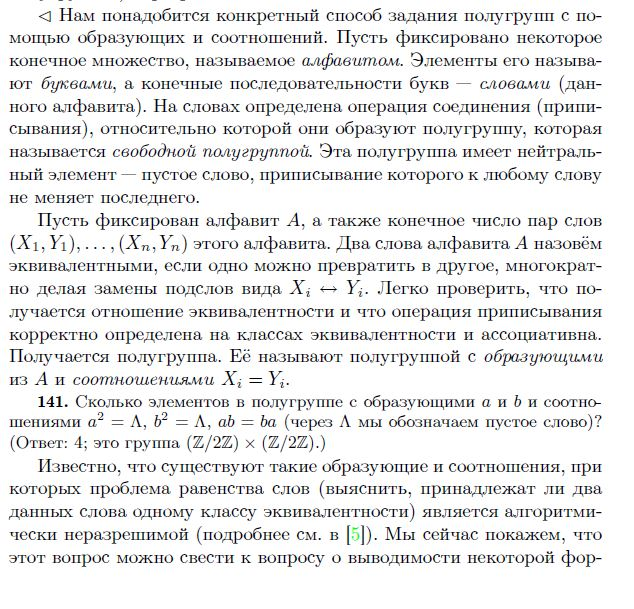
\includegraphics[width=0.48\textwidth]{images/1.1_church1}
    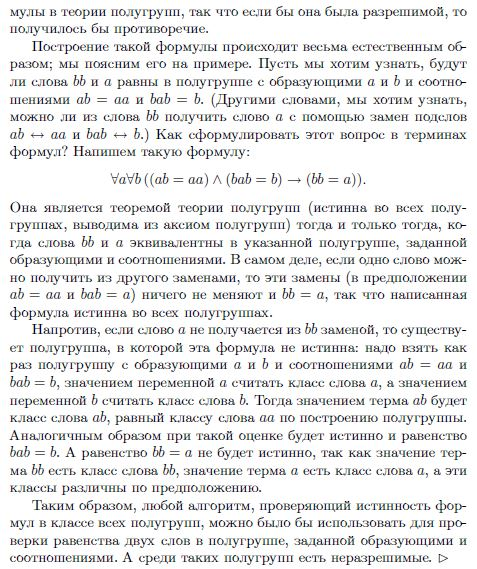
\includegraphics[width=0.48\textwidth]{images/1.1_church2}
\end{center}

\textbf{Теорема Чёрча}. Не существует алгоритма, проверяющего общезначи-
мость формул первого порядка.

В этой формулировке не ограничивается сигнатура (от алгоритма требуется, чтобы он определял общезначимость формулы с произвольным числом предикатных и функциональных символов). На
самом деле неразрешимость возникает уже в совсем простых сигнатурах, как видно из доказательства.

$\blacktriangle$
Поскольку теория полугрупп конечно аксиоматизируема, то выводимость формулы F в этой теории равносильна общезначимости формулы $A \rightarrow F$, где A — конъюнкция всех аксиом теории полугрупп.
$\blacksquare$